\documentclass[twocolumn,fontsize=11pt]{scrartcl}

% Basic packages
\usepackage[utf8]{inputenc}
\usepackage[T1]{fontenc}
\usepackage{lmodern}
\usepackage[a4paper,margin=1.5cm]{geometry}
\usepackage{multicol}
\usepackage{graphicx}
\usepackage{caption}
\usepackage{subcaption}
\usepackage{amsmath,amssymb}
\usepackage{siunitx}
\usepackage{booktabs}
\usepackage{physics}
\usepackage{float}
\usepackage{csquotes}
\usepackage{hyperref}
\usepackage{physics_macros} % Your custom macros
\usepackage{biblatex} % For bibliography
\addbibresource{bibliography.bib}

% Header and footer
\usepackage{fancyhdr}
\pagestyle{fancy}
\fancyhf{}
\lhead{Star and Stellar Evolution}
\rhead{\thepage}

%Folder
\graphicspath{{plots/}}

% Title
\title{\vspace{-1cm}Stellar Structure Evolution with MESA}
\author{Bruno da Rocha Schultz}
\date{\today}

\begin{document}
\maketitle

\section*{Exercise 1}

\paragraph{Q.1.1:} Why is there only one history file but multiple profile files?

\paragraph{A:} The history file contains the global properties of the star at each time step, while the profile files contain the detailed structure of the star at specific points in time. The history file is updated at each time step, but the profile files are only written at certain intervals. So there is one history file for the entire simulation, but multiple profile files corresponding to different time steps.

\paragraph{Q.1.2:} Show with a plot whether or not the size of the time steps in the history file changes
during the simulation, and discuss why.

\paragraph{A:} The time steps in the history file do change during the simulation. This is because MESA uses an adaptive time-stepping algorithm to ensure that the simulation progresses at a rate that captures the important changes in the star's structure and evolution. The time steps are smaller during rapid changes (like during a shell flash) and larger during more stable phases. Cf. Figure \ref{fig:time_steps} for a plot of the time steps recorded in the history file. 

\begin{figure}[htbp]
    \centering
    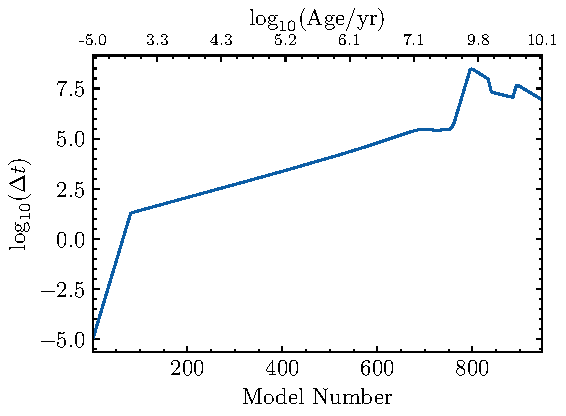
\includegraphics{log_dt_vs_model_number.pdf}
    \caption{Time steps recorded in the history file. The x-axis shows the model number (bottom) and the logarithm of the stellar age (top). The y-axis shows the logarithm of the time step size.}
    \label{fig:time_steps}
\end{figure}

\paragraph{Q.1.3:} Similarly, show with a plot whether or not the grid spacing in a profile file of your
choice is constant, and discuss why. From this plot, also infer which zone is the most  
central zone (zone number 1 or the zone with the highest number).

\paragraph{A:} The grid spacing in a profile file is not constant. MESA uses a non-uniform grid so it can better capture important changes inside the star, making the grid finer where the structure changes quickly and coarser where things are more uniform. In Figure \ref{fig:grid_spacing}, the top graph shows that zone number 1 is at the surface, while the highest zone number is at the center. The bottom graph shows that the spacing between zones (measured as \(\log_{10}(\Delta R / R)\)) is not the same everywhere, confirming that the grid is not evenly spaced. Here, \(\Delta R\) is the difference in radius between adjacent zones, i.e. \(\Delta R = R_{i+1} - R_i\).
%
\begin{figure}[htbp]
    \centering
    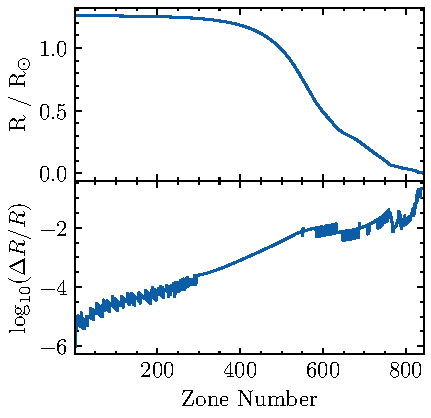
\includegraphics{R_vs_zone.pdf}
    \caption{Grid spacing in a profile file. The x-axis shows the zone number. Top: The radius of each zone.}
    \label{fig:grid_spacing}
\end{figure}
%
\paragraph{Q.1.4:} Which burning stages did the simulation go through, and where did that burning take
place? Graphically Illustrate your answer

\paragraph{A:} Only after the star reaches the zero-age main sequence (the point where the nuclear luminosity exceeds \(99\%\) of the total luminosity, \(\sim 4 \times 10^7\)), is there significant hydrogen burning. Due to the imposed limit \texttt{he\_core\_mass\_limit=0.1}, the star does not reach the conditions necessary for helium burning. To illustrate this,
Figure \ref{fig:q14_luminosity} displays the evolution of hydrogen and helium burning luminosities as the star ages. After the star reaches the ZAMS, hydrogen burning is significant, while helium burning remains negligible for the entire simulation. To indicate where hydrogen burning takes place, Figures \ref{fig:q14_abundancy_H} and \ref{fig:q14_abundancy_e} show the abundances of hydrogen and helium as functions of mass coordinate and stellar age for different late-stage profiles. These plots demonstrate that hydrogen burning is confined to the innermost \(\lesssim 0.15 \text{M}_\odot\) throughout the simulated period.

\begin{figure}[htbp]
    \centering
    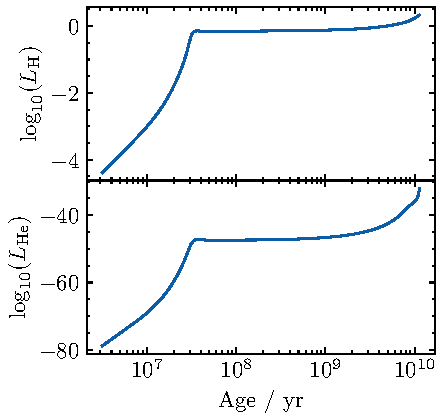
\includegraphics{q14_luminosity.pdf}
    \caption{Hydrogen and helium burning luminosities as a function of stellar age.}
    \label{fig:q14_luminosity}
\end{figure}
\begin{figure}[htbp]
    \centering
    
\includegraphics{q14_abundancy_H.pdf}
    \caption{Hydrogen abundance as a function of mass coordinate and stellar age. The colorbar indicates the hydrogen mass fraction. Hydrogen burning occurs in the core, where the abundance decreases over time.}
    \label{fig:q14_abundancy_H}
\end{figure}
\begin{figure}[htbp]
    \centering
    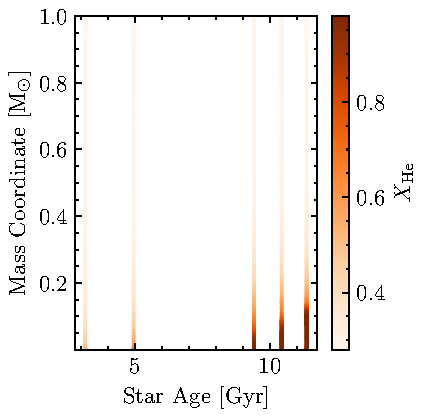
\includegraphics{q14_abundancy_He.pdf}
    \caption{Helium abundance as a function of mass coordinate and stellar age. The colorbar indicates the helium mass fraction. Helium accumulates in the core as hydrogen is fused.}
    \label{fig:q14_abundancy_e}
\end{figure}
\paragraph{Q.1.5:} During the evolution of the stellar model, on what timescales does contraction or expansion occur? You can estimate the contraction/expansion timescale as \(\left|R/\dot{R}\right|\). Show this in a plot with \texttt{model\_number} on the x-axis. Furthermore, show the evolution of the three timescales mentioned above in this plot, and explain in your answer how you defined them. Discuss why the model follows certain timescales during different phases of the simulation.

\paragraph{A:} The contraction or expansion timescale can be estimated as \(\left|R/\dot{R}\right|\), where \(R\) is the radius of the star and \(\dot{R}\) is the time derivative of the radius. The evolution of the contraction/expansion timescale can be plotted against the model number, showing how the star's size changes over time, cf. Figure \ref{fig:q14_timescales}. We calculate the timescales of stellar evolution as follows:
\begin{align*}
    \tau_{\text{dyn}} &\simeq 0.02 \left(\frac{R}{\Rsun}\right)^{3/2} \left(\frac{\Msun}{M}\right)^{1/2} \text{days}, \\
    \tau_{\text{KH}} &\simeq 1.5 \times 10^7\left(\frac{M}{\Msun}\right)^{2} \frac{\Rsun}{R}\frac{\Lsun}{L} \text{years}, \\
    \tau_{\text{nuc}} &\simeq \times 10^{10}\left(\frac{M}{\Msun}\right)\left(\frac{\Lsun}{L}\right)
\end{align*}
During the pre-main sequence phase, the star contracts under gravity, causing its radius to decrease. As this happens, the dynamical timescale (\(\tau_{\text{dyn}}\)), which measures how quickly the star can adjust to changes in structure, becomes shorter because a more compact star responds faster (\(\tau_{\text{dyn}} \propto R^{3/2}\)). The Kelvin-Helmholtz timescale (\(\tau_{\text{KH}}\)), which is the time it takes the star to radiate away its gravitational energy and reach thermal equilibrium, increases as the star contracts and its luminosity drops as it goes down the Hayashi track (\(\tau_{\text{KH}} \propto R^{-1} L^{-1}\)). The nuclear timescale (\(\tau_{\text{nuc}}\)), representing how long the star can sustain nuclear burning, also increases with the decreasing luminosity \(\tau_{\text{nuc}} \propto L^{-1}\). Upon reaching the zero-age main sequence (ZAMS), hydrogen fusion in the core becomes dominant. At this stage, the star and the timescales stabilizes staying at the same order of magnitude. The dynamical timescale remains short at about \(30 \text{min}\), the Kelvin-Helmholtz timescale stays roughly at \(10^7\) yr, and the nuclear timescale is \(10^{10}\) yr. Only as the star starts exiting the main sequence does the internal structure and thus the timescales change again. The core contracts and the outer envelope expands, increasing both the radius and luminosity. These changes cause the dynamical to increase, while the Kelvin-Helmholtz and nuclear timescale decreases due to the enhanced luminosity. Cf. Figure \ref{fig:q15_timescales}.
\begin{figure}[htbp]
    \centering
    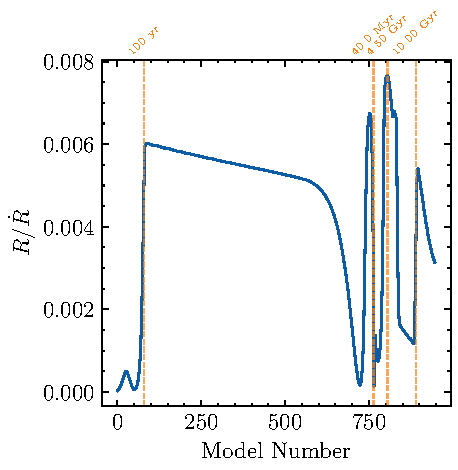
\includegraphics{R_dot_vs_model_number.pdf}
    \caption{Contraction/expansion timescale. The x-axis shows the model number, while the y-axis shows the timescales in years. For clarity, the star age is also shown on the top x-axis.}
    \label{fig:q14_timescales}
\end{figure}
\begin{figure}[htbp]
    \centering
    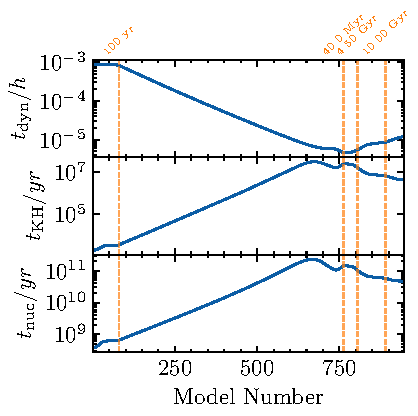
\includegraphics{timescales_vs_model_number.pdf}
    \caption{Evolution of the dynamical timescale, Kelvin-Helmholtz timescale, and nuclear timescale as a function of model number. The x-axis shows the model number, while the y-axis shows the timescales. }
    \label{fig:q15_timescales}
\end{figure}
\clearpage
\section*{Exercise 2}

\paragraph{Q2.1:} In terms of relative mass coordinate \(q\), what parts of your star are convective at the terminal-age main sequence (TAMS)? Use information about temperature gradients in
a profile to show this in a plot.

\paragraph{A:} To the determine which part of the star is convective at the terminal-age main sequence (TAMS), we can look at the temperature gradient in a profile file. The Schwarzschild criterion states that convection occurs when the temperature radiative gradient is steeper than the adiabatic gradient. In Figure \ref{fig:q21_convective_regions}, we plot the temperature gradients as a function of the relative mass coordinate for a star with \(M = 8.655\Msun\). We can see that the star is convective whithin the central grey-colored region (\(q \lesssim 0.09\)).

\begin{figure}[htbp]
    \centering
    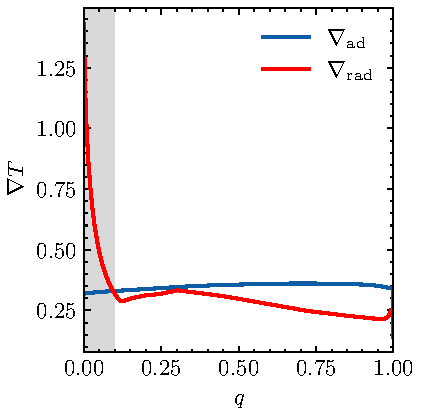
\includegraphics{q21_grad.pdf}
    \caption{Temperature gradients as a function of relative mass coordinate (\(q\)) at the TAMS. The convective region is where the radiative gradient (\(\nabla_{\text{rad}}\)) exceeds the adiabatic gradient (\(\nabla_{\text{ad}}\)), indicated by the shaded area.}
    \label{fig:q21_convective_regions}
\end{figure}

\paragraph{Q2.2:} Show, in an initial mass (x-axis) vs. \(q\) (y-axis) plot, which parts of the stars simulated by you and your colleagues are convective at TAMS. Briefly explain: i) the behavior as a function of mass, and ii) the main difference to the shaded region in fig. 8.8 of the SSE lecture notes and where this difference arises from.

\paragraph{A:} In Figure \ref{fig:q22_convective_regions}, we plot the convective regions at TAMS for stars with different initial masses. The x-axis shows the initial mass of the star, while the y-axis shows the maximum relative mass coordinate at which the star is convective \(q_\text{top}\). We can see that the convective region increases roughly linearly with the initial mass of the star. This trend arises because higher-mass stars generate most of their energy via the CNO cycle, which is highly temperature-sensitive. This leads to a steep radiative temperature gradient in the core, triggering convection over a more extended region for more massive stars. The main difference to the shaded region in Figure 8.8 of the SSE lecture is simply the fact that we are looking at the convective regions at TAMS, while the shaded region in the lecture notes shows the convective regions at the ZAMS. Convective regions at the ZAMS are generally larger than at TAMS. As the star evolves on the main sequence and the core becomes enriched in helium, the mean molecular weight increases, reducing the radiative gradient. This causes the convective core to shrink, so the convective region at TAMS is typically smaller than at ZAMS.

\begin{figure}[htbp]
    \centering
    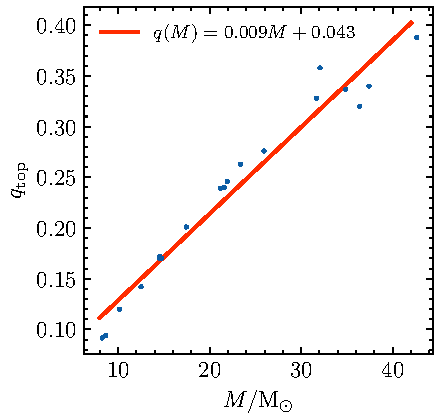
\includegraphics{q22_top_fit.pdf}
    \caption{Convective regions at TAMS for stars with different initial masses. The x-axis shows the initial mass of the star, while the y-axis shows the relative mass coordinate within which the star is convective.}
    \label{fig:q22_convective_regions}
\end{figure}

\paragraph{Q2.3:} Create an HR diagram that shows both stars that you simulated in this exercise. Show the points where they exhaust hydrogen in their cores. After H-exhaustion, is the change in \(\log(L/L_\odot)\) the same in both stars? Why (not)? 

\paragraph{A:} In Figure \ref{fig:q23_H_burning}, we plot the HR diagram for the two stars simulated in this exercise \(M_1 = 8.655\Msun\) and \(M_2 = 1.645\Msun\). The points where they exhaust hydrogen in their cores are marked with red circles. After hydrogen exhaustion, the change in \(\log(L/L_\odot)\) is not the same for both stars. The lower-mass star experiences a more dramatic increase in luminosity. After core hydrogen is exhausted, it develops a degenerate helium core and continues hydrogen burning in a shell. This leads the star to ascend the red giant branch, during which the envelope expands and the luminosity increases steeply. The higher-mass stars core does not become degenerate, and it transitions more smoothly to core helium burning. While its luminosity also increases, the change in \(\log(L/L_\odot)\) is less steep compared to the low-mass star.

\begin{figure}[htbp]
    \centering
    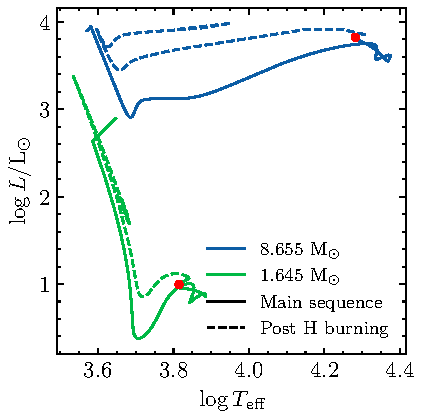
\includegraphics{q23_H_burning.pdf}
    \caption{HR diagram for the two stars simulated in this exercise. The red circles indicate the points where the stars exhaust hydrogen in their cores.}
    \label{fig:q23_H_burning}
\end{figure} 

\paragraph{Q2.4:} Draw the tracks of your evolutionary models computed in this exercise in a \(\log T_c\)–\(\log \rho_c\) diagram, and identify the key differences between the two. Draw the dashed lines of Fig. 3.4 in the SSE lecture notes in your plot, and explain how you drew them.

\paragraph{A:} In Figure \ref{fig:q24_deg}, we plot the tracks of the two evolutionary models in a \(\log T_c\)-\(\log \rho_c\) diagram. The x-axis shows the logarithm of the central temperature, while the y-axis shows the logarithm of the central density. The dashed lines in the plot were drawn using the analytical expressions given in Figure 3.4 of the SSE lecture notes. Each line corresponds to a boundary where different pressure components become dominant: radiation vs.\ gas pressure (black, slope \(1/3\)), gas vs.\ non-relativistic degeneracy (red, slope \(2/3\)), gas vs.\ relativistic degeneracy (yellow, slope \(1/3\)), and the transition between non-relativistic and extremely relativistic degeneracy (blue, vertical at \(\log \rho \approx 6.3\)).  These boundaries were derived by equating the relevant equations of state as described in the lecture notes. They help classify which pressure component governs the stellar core at different evolutionary stages. Both tracks start similar, only shifted vertically due to their different masses. As the stars evolve, they follow different paths in the diagram. The higher-mass star (\(8.655\,\Msun\)) remains above the non-relativistic degeneracy line, while the lower-mass star (\(1.645\,\Msun\)) approaches the relativistic degeneracy line as it evolves.
The $8.655\,\Msun$ track (blue) moves to higher central temperatures ($T_c$) and avoids degeneracy. The $1.645\,\Msun$ track (green) starts curving around the degenerate region.

\begin{figure*}[p]
    \centering
    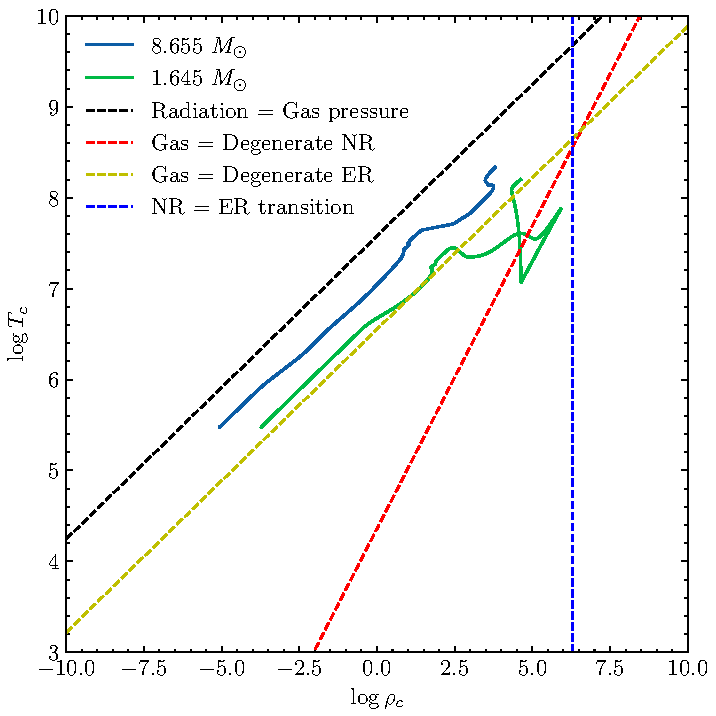
\includegraphics{q24_deg.pdf}
    \caption{Tracks of the two evolutionary models in the \(\log T_c\)-\(\log \rho_c\) diagram. The dashed lines correspond to the boundaries between different stellar evolutionary phases, as in Fig. 3.4 of the SSE lecture notes.}
    \label{fig:q24_deg}
\end{figure*}
\clearpage
\section*{Exercise 3}

\paragraph{Q3.1:} Does MESA use the Schwarzschild or Ledoux criterion for convection by default? 

\paragraph{A:} MESA uses the Schwarzschild criterion by default, as can be confirmed by looking in the documentation. 

\paragraph{Q3.2:} How many millions of years (Myr) do H and He core burning last?

\paragraph{A:} With an overshooting parameter of \(0.121\), the duration of core hydrogen burning is approximately \(11.55\) Myr, and core helium burning lasts about \(1.16\) Myr. These timescales are estimated from the history file by locating the stellar ages when \texttt{center\_h1} becomes zero and when \texttt{center\_he4} decreases to roughly 0.01 (marking the end of core helium burning). See Figure \ref{fig:q31_core_burning} for a graphical representation of these phases.
\begin{figure}[htbp]
    \centering
    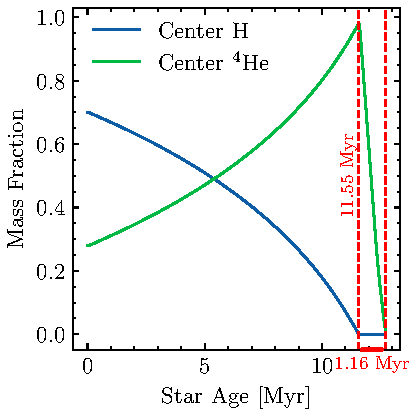
\includegraphics{q31center_h_he.pdf}
    \caption{Core burning phases. The x-axis shows the stellar age, while the y-axis shows the central hydrogen and helium abundances. The red dashed lines indicate the end of hydrogen burning and the end of helium burning.}
    \label{fig:q31_core_burning} 
\end{figure}   

\paragraph{Q3.3:} Show graphically how overshooting affects the core hydrogen and the core helium burning lifetimes. Explain why.

\paragraph{A:} Figure~\ref{fig:q31core_burning_lifetime}, plots the core hydrogen and helium burning lifetimes as a function of the overshooting parameter \(\alpha_{\mathrm{ov}}\). Linear fits are shown for both burning phases:
\begin{align*}
    \tau_{\mathrm{H}} &= 7.01\,\alpha_{\mathrm{ov}} + 10.68\ \text{Myr}, \\
    \tau_{\mathrm{He}} &= -1.35\,\alpha_{\mathrm{ov}} + 1.29\ \text{Myr}.
\end{align*}
We find that the hydrogen-burning lifetime increases significantly with higher overshooting, while the helium-burning lifetime decreases slightly. This trend can be understood since increased overshooting extends the size of the convective core during the main sequence, allowing more hydrogen to be mixed into the core. As a result, hydrogen burning lasts longer. This leads to a more massive helium core after hydrogen exhaustion, which in turn evolves more quickly during helium burning. The larger and hotter He core burns through its fuel more rapidly, resulting in a shorter He-burning phase.
\begin{figure}[htbp]
    \centering
    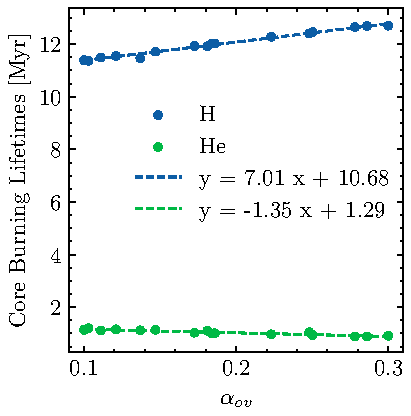
\includegraphics{q31core_burning_lifetime.pdf}
    \caption{Core hydrogen and helium burning lifetimes as a function of the overshooting parameter \(\alpha_{\mathrm{ov}}\). The blue line shows the core hydrogen burning lifetime, while the green line shows the core helium burning lifetime. The dashed lines are linear fits to the data points.}
    \label{fig:q31core_burning_lifetime}
\end{figure}

\paragraph{Q3.4:} For the first profile before hydrogen is exhausted in the core (which happens when, say, \(X_c < 10^{-6}\)) and for the first profile after that, plot the H and He abundances as a function of mass coordinate. Do this for both the Ledoux and the Schwarzschild simulation. For which simulation did the abundance profile change more dramatically, and why?

\paragraph{A:} In Figure~\ref{fig:q34hydrogen_exhausted}, we compare the hydrogen and helium abundance profiles before and after core hydrogen exhaustion for both the Schwarzschild and Ledoux simulations of a $15\Msun$ star. We find that the abundance profiles change more dramatically in the Schwarzschild simulation. After core hydrogen exhaustion, the Schwarzschild model exhibits a noticeable step-like structure in the hydrogen and helium mass fractions. This results from the fact that the Schwarzschild criterion for convection does not account for stabilizing composition gradients \(\nabla_\mu\). It only considers the temperature gradient when determining convective instability. As a result, convective mixing penetrates farther into surrounding layers, even when a chemical gradient is present. In contrast, the Ledoux simulation shows a much more gradual and limited change in composition, with a smooth transition between H-rich and He-rich regions. This is because the Ledoux criterion includes the stabilizing effect of mean molecular weight gradients, reducing mixing. In stellar interiors, molecular weight typically increases toward the center due to nuclear processing. Therefore, the gradient \(\nabla_\mu > 0\) suppresses convection in Ledoux criterion. This makes sense, since an upwardly displaced fluid element from a deeper layer will have a higher molecular weight (i.e., more heavy elements) than its surroundings. Even if it is hotter, the increased molecular weight makes it denser overall, causing a restoring force to push it back downward. Thus, the Ledoux criterion prevents convection in regions where the Schwarzschild criterion would otherwise allow it, leading to less mixing and smoother abundance profiles.

\begin{figure}
    \centering
    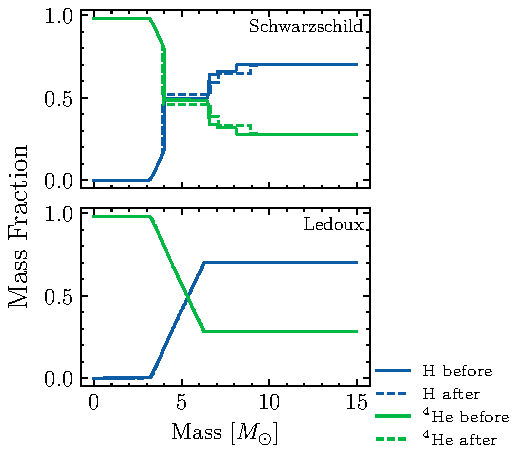
\includegraphics[width=0.49\textwidth]{q34hydrogen_exhausted.pdf}
    \caption{Hydrogen and helium abundance profiles before and after core hydrogen exhaustion for the Schwarzschild and Ledoux simulations.}
    \label{fig:q34hydrogen_exhausted}   
\end{figure}

\clearpage
\section*{Exercise 4}

\paragraph{Q4.1:} What extra isotopes are included in this network using? Look for clues in the folder \texttt{\$MESA\_DIR/data/net\_data/nets}.

\paragraph{A:} The \texttt{pp\_extras} network includes the standard isotopes from the basic pp-chain network \textsuperscript{1}H, \textsuperscript{3}He, \textsuperscript{4}He, \textsuperscript{12}C, \textsuperscript{14}N, \textsuperscript{16}O, \textsuperscript{20}Ne, \textsuperscript{24}Mg  and adds extra isotopes \textsuperscript{2}H, \textsuperscript{7}Li, \textsuperscript{7}Be, \textsuperscript{8}B.

\paragraph{Q4.2:} Compare the pre-MS (i.e., before 4He is synthesized from hydrogen) radius evolution
of this simulation with that of the low-mass star in Exercise 2. Is there any difference?
If so, provide a plot that shows the different behavior, and explain what caused it.

\paragraph{A:} We use a profile interval of 25 for both simulations. There is a noticeable difference in the pre-main sequence (pre-MS). The key difference is the presence of a \enquote{deuterium bump} in the radius evolution, visible as a temporary halt or even slight increase in radius at an age of about \(10^5\) years (see Figure~\ref{fig:q42_radius_vs_age}). Deuterium is a very fragile nucleus that reacts easily with normal hydrogen (\(^{2}\mathrm{H} + ^{1}\mathrm{H} \rightarrow ^{3}\mathrm{He} + \gamma\)), the second reaction in the pp chain. This reaction destroys all deuterium present in the star when \(T \approx 10^6\,\mathrm{K}\), while the protostar is still on the Hayashi line. The energy produced is large enough to halt the contraction of the PMS star for a few times \(10^5\) yr.
\begin{figure}[htbp]
    \centering
    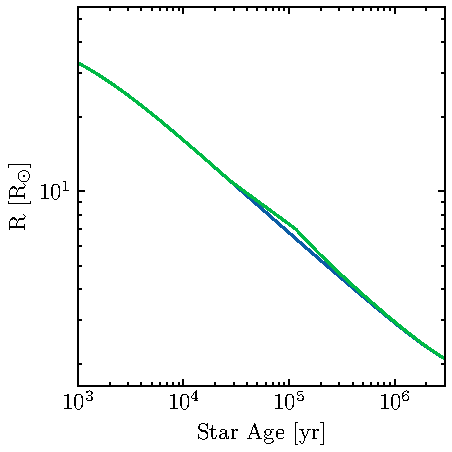
\includegraphics{q42_radius_vs_age.pdf}
    \caption{Pre-main sequence radius evolution showing the deuterium bump at around \(10^5\) years. The temporary halt in contraction is caused by deuterium burning.}
    \label{fig:q42_radius_vs_age}
\end{figure}

\paragraph{Q4.3:} \textsuperscript{2}H undergoes nuclear burning around \(10^6\,\mathrm{K}\). Once \textsuperscript{2}H burning starts, graphically show whether the \textsuperscript{2}H abundance decreases everywhere in the star at roughly the same time, or only locally. Explain why this happens.

\paragraph{A:} We select only those models where \(T > 10^6\,\mathrm{K}\). At around \(10^6\,\mathrm{K}\), \textsuperscript{2}H burning begins in the star's core where the temperature is highest. Because the star is fully convective up to about \(0.6\) Myr, convection rapidly mixes material throughout the interior. This efficient mixing transports \textsuperscript{2}H from the outer layers into the burning region and redistributes depleted material outward, causing the \textsuperscript{2}H abundance to decrease almost uniformly throughout the convective zone. Thus, the \textsuperscript{2}H abundance drops nearly simultaneously everywhere, showing a flat radial profile that declines over time. After convection ceases or weakens, depletion becomes more localized near the core. Cf. Figure~\ref{fig:q42_h2_profile} for the \textsuperscript{2}H abundance profile at different times. 

\begin{figure}[htbp]
    \centering
    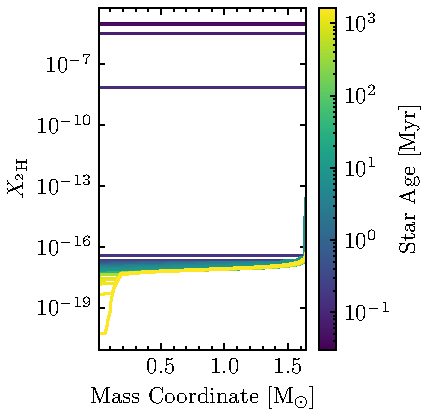
\includegraphics{q42_h2_profile.pdf}
    \caption{\textsuperscript{2}H abundance profiles at various times. The x-axis represents the mass coordinate, and the y-axis shows the \textsuperscript{2}H abundance. The colorbar indicates the star age. Initially, the \textsuperscript{2}H abundance decreases uniformly across the convective zone, resulting in a flat profile that declines over time.}
    \label{fig:q42_h2_profile}
\end{figure}

\paragraph{Q4.4:} Use Python to draw an integer \(k\) from the list \([2, 3, 5, 7]\) using the line
\begin{verbatim}
numpy.random.choice([2, 3, 5, 7])
\end{verbatim}
What value did you draw for \(k\)? Now assume we live in a different universe, where \(^2\mathrm{H}\) burns at \(k \times 10^6\,\mathrm{K}\) instead of \(10^6\,\mathrm{K}\). In that case, for the stellar model you ran in this exercise, would you expect \(^2\mathrm{H}\) to be absent in every layer once it is exhausted in the center of the star? Use a plot to motivate your answer.

\paragraph{A:} In our new universe, \(^2\mathrm{H}\) burns at \(2 \times 10^6\,\mathrm{K}\). At this higher temperature, deuterium burning begins later, when the star is less convective. As a result, \(^2\mathrm{H}\) is depleted primarily in the core, while the outer layers retain higher abundances. This leads to a non-uniform \(^2\mathrm{H}\) profile, with a step-wise depletion in the core as the outer layers slowly heat up to the required temperature to burn deuterium . In Figure \ref{fig:q42_h2_profile_new_universe}, we plot the \(^2\mathrm{H}\) abundance profiles in this alternate universe. The profile shows that while the core is depleted, the outer layers still contain significant amounts of \(^2\mathrm{H}\), indicating that it is not uniformly absent throughout the star.

\begin{figure}[htbp]
    \centering
    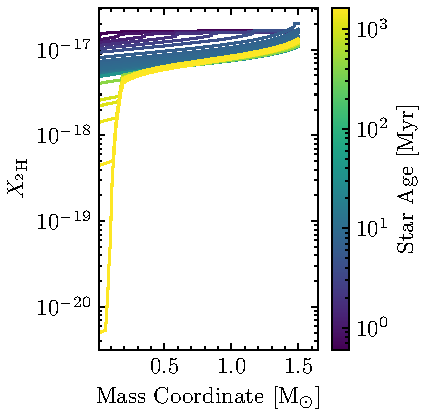
\includegraphics{q42_h2_profile_new_universe.pdf}
    \caption{\(^2\mathrm{H}\) abundance profiles in the alternate universe where deuterium burns at \(5 \times 10^6\,\mathrm{K}\). The abundance is depleted in the core but remains high in the outer layers, showing non-uniform depletion.}
    \label{fig:q42_h2_profile_new_universe}
\end{figure}

\printbibliography

\end{document}
